% https://tex.stackexchange.com/a/470208
\documentclass[aspectratio=169]{beamer}
\usepackage{tikz}
\usepackage{circuitikz}


\begin{document}

\begin{frame}{Question}


\begin{columns}[onlytextwidth]
\begin{column}{0.5\textwidth}
\begin{figure}
%\begin{center}
\begin{circuitikz}

\draw (0,0)
to[short](0,3) coordinate[label=above:$D$] (D)
to[short](3,3) coordinate[label=above:$C$] (C)
to[short](3,0) coordinate[label=above:$G$] (G)
to[short](0,0) coordinate[label=above:$H$] (H)
(1,2)
to[short](4,2) coordinate[label=above:$B$] (B)
to[short](4,-1)coordinate[label=above:$F$] (F)
to[short](1,-1)coordinate[label=above:$E$] (E)
to[short](1,2) coordinate[label=above:$A$] (A)
(D) to[short] (A)
(C) to[short] (B)
(H) to[short] (E)
(G) to[short] (F);
\fill[orange,opacity=0.4](A)--(B)--(C)--(D)--cycle;
\fill[red,opacity=0.4](A)--(D)--(H)--(E)--cycle;
\fill[blue,opacity=0.4](B)--(C)--(G)--(F)--cycle;


\end{circuitikz}
%\end{center}
\end{figure}
\end{column}
\begin{column}{0.5\textwidth}
\begin{figure}
%\begin{center}
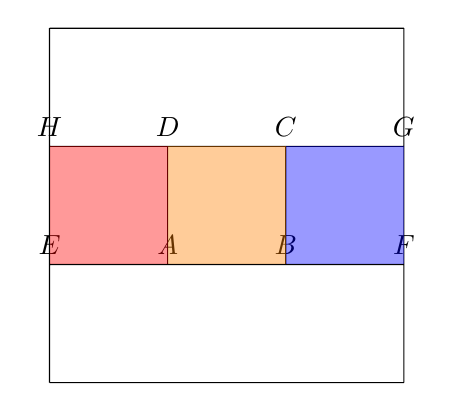
\begin{tikzpicture}[scale=0.3]

\draw (0,2.5)                   coordinate[label=above:$H$] (H)
to[short](15,2.5)               coordinate[label=above:$G$] (G)
(0,-2.5)                        coordinate[label=above:$E$] (E)
to[short](15,-2.5)              coordinate[label=above:$F$] (F)
(0,7.5)
to[short](15,7.5)
(0,-7.5)
to[short](15,-7.5)
(15,7.5)
to[short](15,-7.5)
(0,7.5)
to[short](0,-7.5)
(5,2.5)                        coordinate[label=above:$D$] (D)
to[short](5,-2.5)              coordinate[label=above:$A$] (A)
(10,2.5)                       coordinate[label=above:$C$] (C)
to[short](10,-2.5)             coordinate[label=above:$B$] (B);

\fill[orange,opacity=0.4](A)--(B)--(C)--(D)--cycle;
\fill[red,opacity=0.4](A)--(D)--(H)--(E)--cycle;
\fill[blue,opacity=0.4](B)--(C)--(G)--(F)--cycle;


\end{tikzpicture}
%\end{center}
\end{figure}
\end{column}
\end{columns}

\end{frame}

\end{document}
